\chapter{Практическая часть}

Проанализировать работу приведенных программ и объяснить результат их работы.

\section{Задание \No{}1}
Первая программа:
\lstset{language=c}
\begin{lstlisting}[caption=Текст программы первого задания]
#include <stdio.h>
#include <fcntl.h>

int main()
{
    int fd = open("alphabet.txt", O_RDONLY);

    FILE *fs1 = fdopen(fd, "r");
    char buff1[20];
    setvbuf(fs1, buff1, _IOFBF, 20);

    FILE *fs2 = fdopen(fd, "r");
    char buff2[20];
    setvbuf(fs2, buff2, _IOFBF, 20);

    int flag1 = 1, flag2 = 2;

    while(flag1 == 1 || flag2 == 1)
    {
        char c;

        flag1 = fscanf(fs1, "%c", &c);
        if (flag1 == 1)
            fprintf(stdout, "%c", c);

        flag2 = fscanf(fs2, "%c", &c);
        if (flag2 == 1)
            fprintf(stdout, "%c", c);
    }

    return 0;
}
\end{lstlisting}

~\

Результат:
\begin{figure}[H]
    \centering
    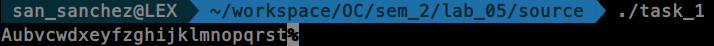
\includegraphics[scale=0.5]{data/image/task_1.png}
    \caption{Скришот результата работы первой программы.}
\end{figure}

Системный вызов open() создаёт файловый дескриптор, который открывается только на чтение, указатель устанавливается на начало файла.
В результате чего создаётся запись в общесистемной таблице открытых файлов.

Затем с помощью функции fdopen() создаются два разных объекта структуры FILE, которые ссылаются на один файловый дескриптор fd и setvbuf() устанавливает тип буферизации блоком, размер которого 20 байт.

Далее в цикле происходит чтение и вывод.
Системная фукнция fscanf() возращает -1, если число прочитанных символов равно нулю, и 1 в ином случае.


При первом вызове fscanf() буфер ввода структуры FILE заполняется либо до конца буфера, либо до конца файла. Поэтому буфер заполняется первыми 20 символами и значение текущей позиции смещается.

Так как fs1 и fs2 ссылаются на одну и ту же запись в системной таблице открытых файлов, значение позиции файла одинаковое, из чего следует, что при следующем вызове fscanf() буфер ввода структуры fs2 считает оставшиейся символы из файла.
В результате получается строка, в которой символы чередуются из первого и второго буфера.

\begin{figure}[H]
    \centering
    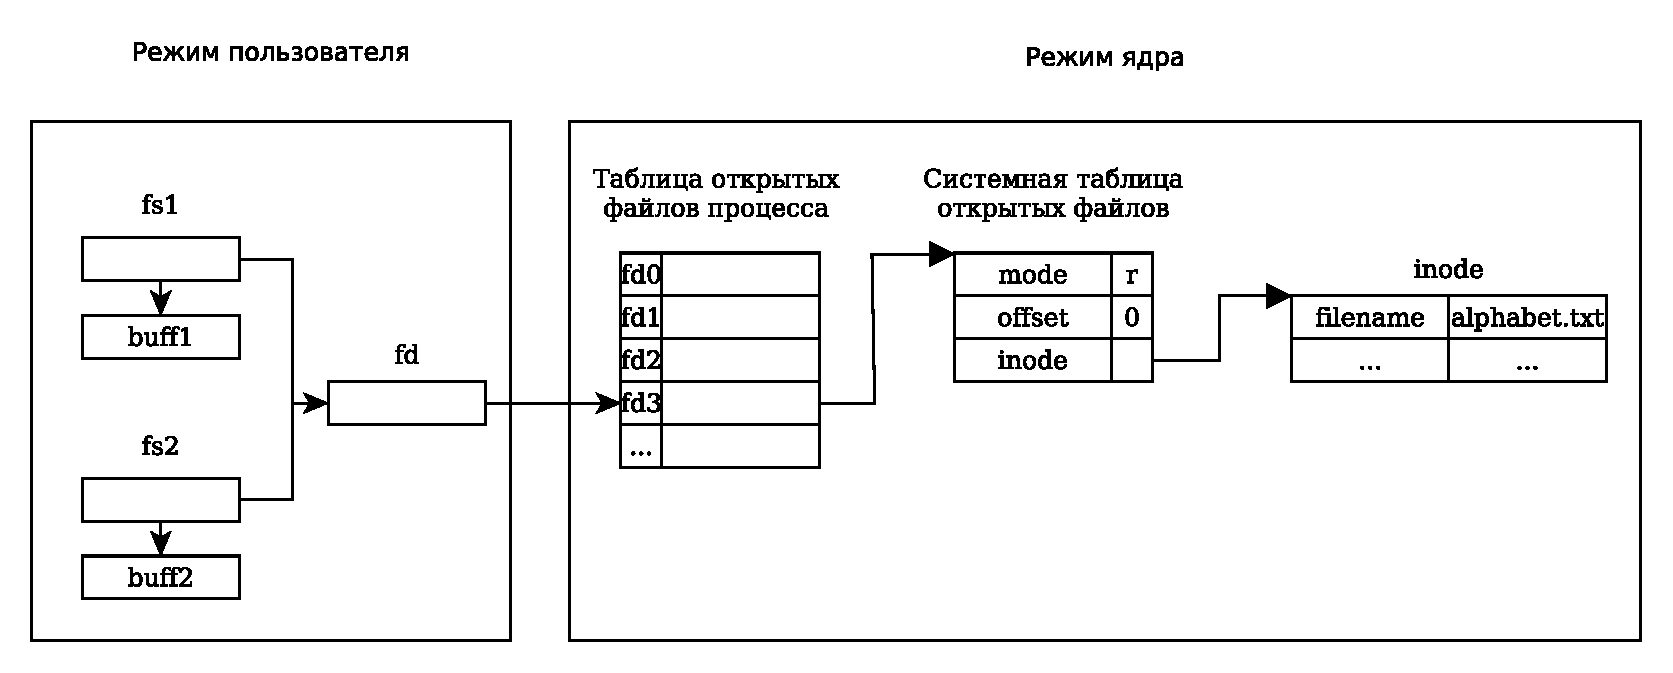
\includegraphics[scale=0.6]{data/pdf/task_1.pdf}
    \caption{Схема связи дескрипторов первой программы.}
\end{figure}

\section{Задание \No{}2}

Вторая программа:
\lstset{language=c}
\begin{lstlisting}[caption=Текст программы второго задания]
#include <stdio.h>
#include <fcntl.h>
#include <unistd.h>

int main()
{
    char c;
    int cond = 1;
    int fd1 = open("alphabet.txt", O_RDONLY);
    int fd2 = open("alphabet.txt", O_RDONLY);

    while(cond)
    {
        if ((cond = read(fd1, &c, 1)) == 1)
        {
            write(1, &c, 1);
        }

        if ((cond = read(fd2, &c, 1)) == 1)
        {
            write(1, &c, 1);
        }
    }

    return 0;
}
\end{lstlisting}

Результат:
\begin{figure}[H]
    \centering
    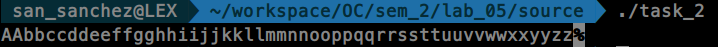
\includegraphics[scale=0.5]{data/image/task_2.png}
    \caption{Скришот результата работы второй программы.}
\end{figure}

Системный вызов open() создаёт 2 разных файловых дескриптора для открытого файла, 2 записи в общесистемной таблице открытых файлов. Так как файловые дескрипторы разные, то у каждого имеется своя текущая позиция файла.
В результате получается строка, в которой символы дублируются.

\begin{figure}[H]
    \centering
    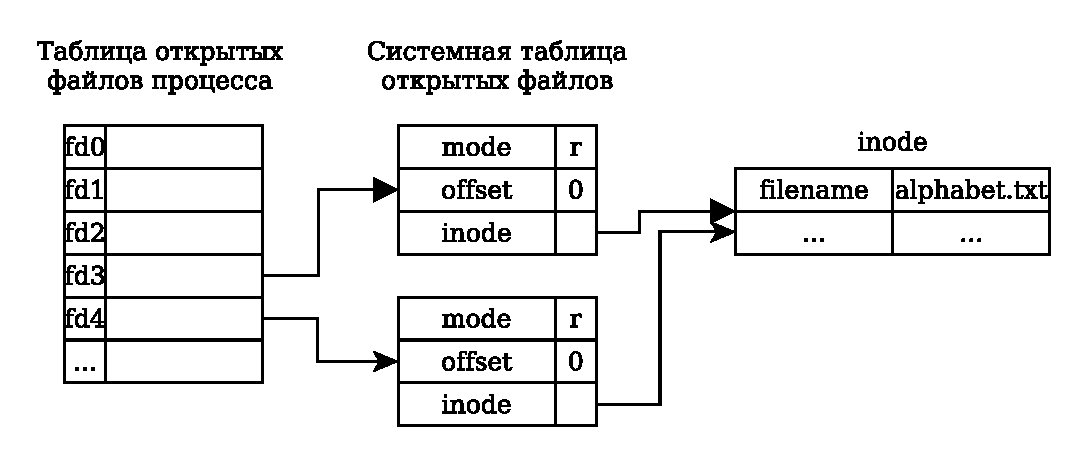
\includegraphics[scale=0.75]{data/pdf/task_2.pdf}
    \caption{Схема связи дескрипторов второй программы.}
\end{figure}

\section{Задание \No{}3}
Написать программу, которая открывает один и тот же файл два раза с использованием
библиотечной функции fopen(). Для этого объявляются два файловых дескриптора. В цикле
записать в файл буквы латинского алфавита поочередно передавая функции fprintf() то
первый дескриптор, то – второй.
Результат прокомментировать.

\lstset{language=c}
\begin{lstlisting}[caption=Текст программы третьего задания]
#include <fcntl.h>
#include <stdio.h>
#include <errno.h>
#include <string.h>

int main()
{
  FILE *fd1 = fopen("task_3.txt", "w");
  if (fd1 == NULL)
  {
    printf("%s", strerror(errno));
    return errno;
  }

  FILE *fd2 = fopen("task_3.txt", "w");
  if (fd1 == NULL)
  {
    printf("%s", strerror(errno));
    return errno;
  }

  for(char c = 'a'; c <= 'z'; c++)
  {
    if (c % 2)
    {
      fprintf(fd1, "%c", c);
    }
    else
    {
      fprintf(fd2, "%c", c);
    }
  }

  fclose(fd1);
  fclose(fd2);

  return 0;
}
\end{lstlisting}

Результат:
\begin{figure}[H]
    \centering
    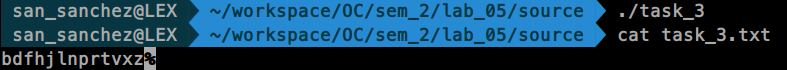
\includegraphics[scale=0.5]{data/image/task_3.png}
    \caption{Скришот результата работы третьей программы.}
\end{figure}

Функция open() создаёт 2 разных файловых дескриптора и две независимые позиции в файле указывают на начало.
Далее в цикле поочередно происходит запись символов от a до z в буферизированные потоки. В первый записываются симовлы на нечётных позициях, а во второй - чётных. Смещение текущей позиции файла независимо для двух различных дескрипторов.
Функция fprintf() выполняет буферизированный вывод - запись в файл происходит при вызове функции fclose(), fflush() или при полном заполнении буфера.
Функция fclose(fd1) очищает поток, на который указывает fd1 (запись любых буферизованных выходных данных с помощью fflush()), и закрывает файловый дескриптор.
Далее выполняется функция fclose(fd2), которая своим выполнением перезапишет данные, записанные fclose(fd1).
В результате получается строка, состоящая из символов английского алфавита, стоящих на чётных позициях.

\begin{figure}[H]
    \centering
    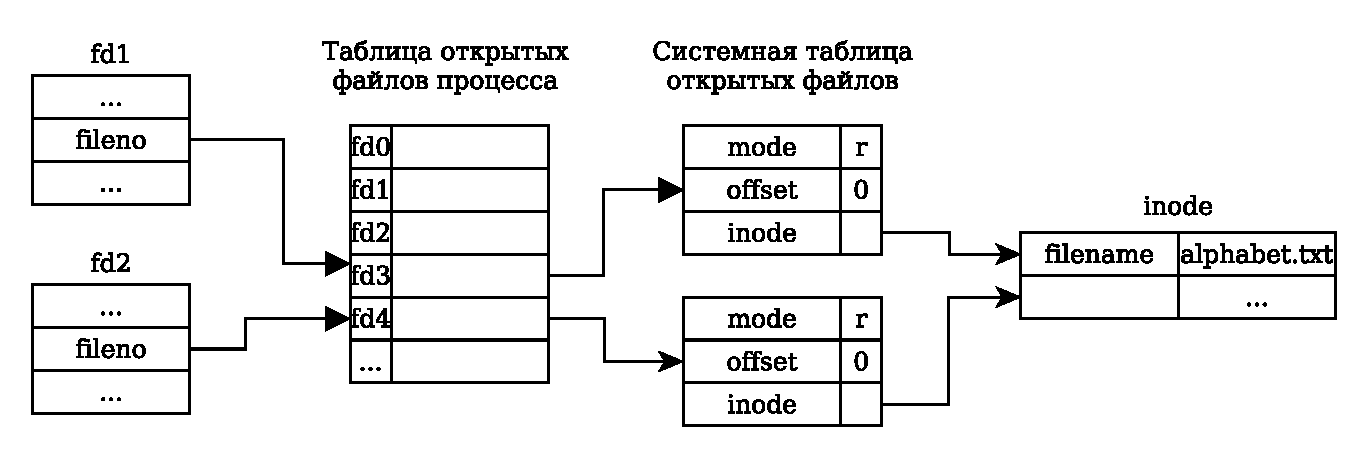
\includegraphics[scale=0.75]{data/pdf/task_3.pdf}
    \caption{Схема связи дескрипторов третьей программы.}
\end{figure}

